\chapter{Vergleich der Implementierungen}
\label{ch:vergleich}
Bisher wurden die Implementierungen nur in einem stationären Szenario mit dem Access Point in Reichweite getestet. 
Dies spiegelt jedoch nicht das Szenario der Arbeit im Tunnel wieder, bei der sich die Mitarbeiter sich regelmäßig bewegen und auch in Bereichen arbeiten, in denen kein AP WLAN zur Verfügung stellt. \\
Ein Test mit den Mitarbeitern war leider nicht möglich, da der Versuchsaufbau mit Powerbank, USB-Power-Meter und ESP8266 Feather zu ausladend und wegen der Steckverbindungen zu fragil für den Arbeitsalltag ist.
Auch das Mitführen des Versuchaufbaus durch den Autor ist nicht praktikabel, da die Versuche über mehrere Stunden durchgeführt werden müssen und in den Arbeitsbereichen auf der Tunnelbohrmaschine nur wenig Platz vorhanden ist, so dass die normale Arbeit behindert werden würde.
Dies ist insbesondere der Fall, wenn realistische Bewegungsprofile nachvollzogen werden sollen. 
Dazu müsste ständig ein Arbeiter verfolgt werden, das behindert diesen natürlich und ist auch nicht einfach möglich, da Gefahrenbereiche vom Autor mangels Sicherheitseinweisungen nicht betreten werden dürften.
Die Bedingungen wurden deshalb stationär simuliert.

\section{Simulationsumgebung}
Für ein realistischen Verbrauch mangelte es der bisherigen stationären Versuchumgebung an Reassiziationen (Wechsel des AP) und dem nicht vorhanden sein eines APs.
Dies soll durch abschalten des APs simuliert werden. \\
Es wurde ein Schema gewählt, in dem der AP nach jeweils 15 Minuten für fünf Minuten abgeschaltet wird. 
Für einen echten Arbeiter sind die Zeitabschnitte anders und je nach Aufgabe unterschiedlich, insbesondere sind die Zeitabschnitte in der Realität länger und die Arbeit außerhalb der Reichweite eines APs wird üblicherweise länger als fünf Minuten dauern.
Weil aber nur ein AP zur Verfügung steht sollen auch Reassoziationen adäquat modelliert werden.
Dies geschiet durch die kurzen Intervalle, da nach dem erneuten anschalten des APs beim Beitreten der mobilen Einheit zum Netzwerk eine Assoziation durchgeführt wird. 
Diese löst, analog zur Reassoziation, einen Sendevorgang bei mobilen Einheiten aus die nur bei Bereichswechsel senden.

\section{Anpassungen der Implementierungen}
Zu Beginn der Tests konnte ein massiver Anstieg des Stromverbrauchs festgestellt werden sobald der AP abgeschaltet wurde.
Geht die Verbindung zu diesem verloren beginnt die mobile Einheit mit einem Scan, in Abschnitt \ref{ch:phase1:sec:wifills} wurde festgestellt, dass diese Operation energetisch sehr teuer ist.
Da der ESP nach einem fehlgeschlagenen Scan sofort einen neuen begann belief sich der Stromverbrauch für Implementierungen, die dem WLAN Netzwerk beitreten, auf 40mA in den Zeiten, in denen der AP abgeschaltet war.
Die Implementierungen wurden daher angepasst, so dass sie nach einem fehlgeschlagenen Scan für das in Abschnitt \ref{ch:Reichweite:sec:bewertung} ermittelte Sendeintervall in den \texttt{deep\_sleep} versetzt werden bevor sie einen neuen Scan starten.
Dieses Verhalten senkt den Energieverbrauch der mobilen Einheiten deutlich.
[Aber trotzdem: Bereichsortung mit TCP Verbindung halten 1,2mA -> 4mA]

\section{Methodik}
Die Methodik zum Messen des Stromverbrauchs wird gegenüber den vorherigen Versuchen verändert.
Der Muker TM103 USB-Power-Meter bietet in seiner Anzeige nur eine geringe zeitliche Auflösung und den Verbrauch des nRF52 konnte er nicht erfassen.\\
Um auch den Verbrauch des nRF52 zu messen und einen genaueren Blick in die Charakteristik des Verbrauchs der anderen Lösungen zu werfen wird stattdessen ein Strommessgerät auf Basis des INA219 verwendet.
Der INA219 kann den Verbrauch mit bis zu 200Hz bestimmen und besitzt dabei eine Messgenauigkeit von 99,5\% \cite{texas2015ina}.
Der Stromverbrauch wird über den Spannungsabfall über einen 0,1$\Omega$ Widerstand bestimmt, der verwendete Widerstand besitzt eine Fertigungstoleranz von 1\%.
Die Messgenauigkeit sinkt deshalb auf $99,5\% * 99\% = 98,505\%$. \\
Außerdem wird dieses mal durch den JST-Anschluss für den Akku gemessen, dadurch können eventuelle Ineffizienzen des Lithium-Polymer-Ladeschaltkreises aufgezeichnet werden. 
Abb. \ref{fig:ina219} zeigt den INA219 integriert auf einer Platine, diese wird für die Messungen verwendet.

\begin{figure}[h]
  \centering
	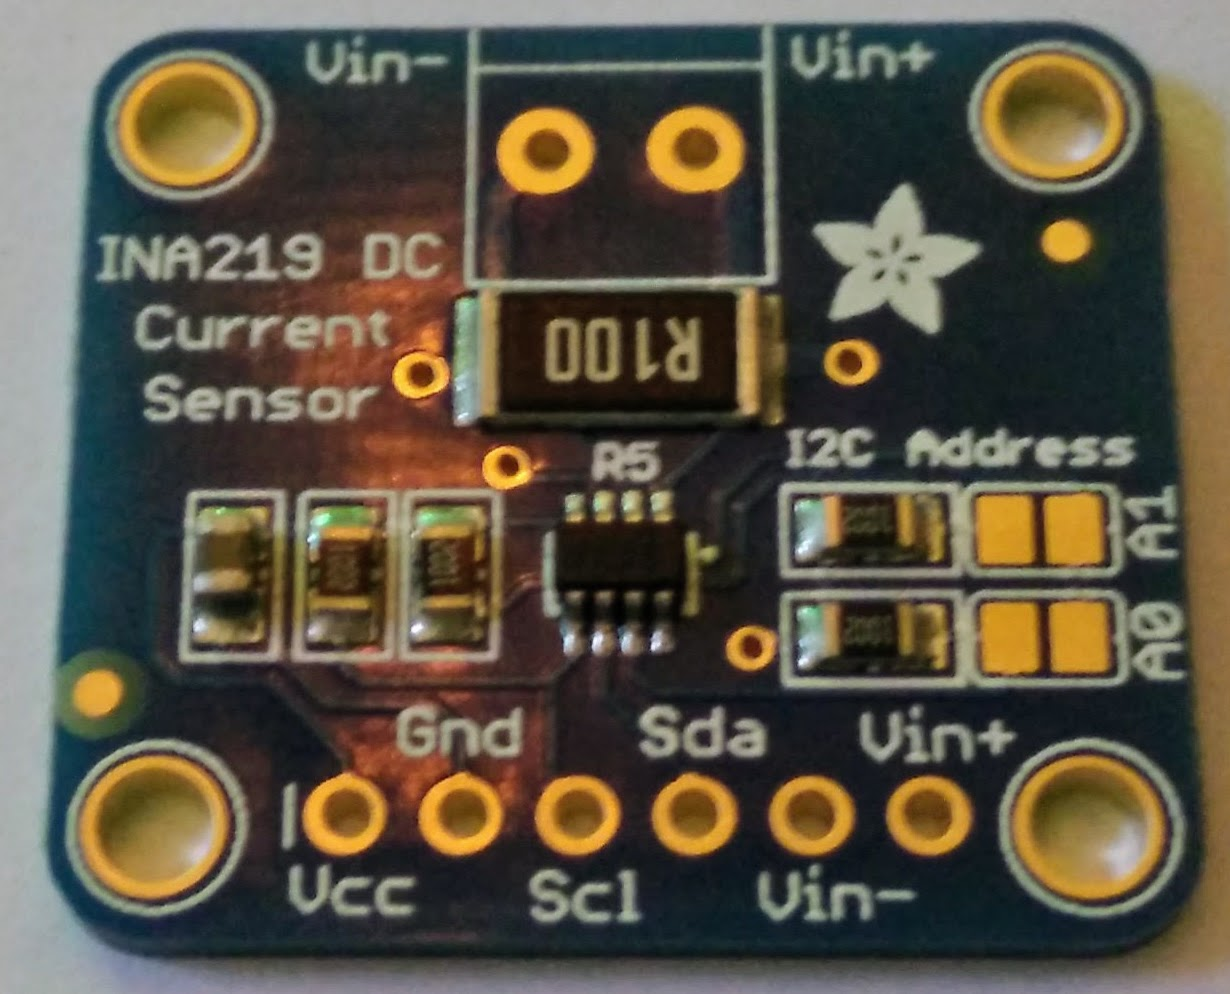
\includegraphics[width=0.5\textwidth]{images/ina219.jpg}
  \caption{INA219, die mit R100 beschriftete Komponente über dem INA219 ist der Messwiderstand.}
  \label{fig:ina219}
\end{figure}

\section{Ergebnisse}
Nachfolgend sind die Ergebnisse für die in dieser Arbeit entstandenen Implementierungen unter den simulierten Bedingungen gelistet.
Es wurde für jedes Konzept jeweils die Implementierung gewählt, die bei den vorherigen Tests innerhalb des Konzepts am besten abgeschnitten hat.\\


\subsection{WiFi-LLS}
\label{ch:realworld:sec:wifills}
Bei WiFi-LLS handelt es sich um mobile Einheiten, die eine Selbstlokalisierung mittels Scan durchführen und die Ergebnisse an einen zentralen Ortungsserver versenden.
Die Implementierung wird in Abschnitt \ref{ch:phase1:sec:wifills} beschrieben.

\subsection{Indirekte Bereichsortung}
\label{ch:realworld:sec:indirekt}
Wegen des hohen Energieverbrauchs der Scan Operation wurde in Abschnitt \ref{ch:phase1:sec:anpassungbereich} eine mobile Einheit beschrieben, die dem Ortungsserver stattdessen nur mitteilt, mit welchem AP sie gerade assoziiert ist. 
Diese Implemetierung wurde optimiert, so dass sie nur sendet, wenn eine Assoziation beziehungsweise Reassoziation stattgefunden hat.

\subsection{RADAR}
Die RADAR Implementierung sendet nach dem Beitritt zum Netzwerk regelmäßig ein 6 Byte langes UDP Paket an den Ortungsserver versendet.
Der Access Point protokolliert den Empfang des Paketes und teilt den Absender dem Ortungsserver mit, zusätzlich wird für eine mögliche Triangulation der Received Signal Strength Index (RSSI) angehängt.
Die Implementierung von RADAR wird in Abschnitt \ref{ch:phase2:sec:radar} beschrieben.

\subsection{Probe Request Lokalisierung}
Die mobile Einheit mit der Probe Request Implementierung sendet regelmäßig den namensgebenden Management Frame aus.
Der Access Point protokolliert den Empfang des Probe Requests und teilt den Absender dem Ortungsserver mit, zusätzlich wird für eine mögliche Triangulation der Received Signal Strength Index (RSSI) angehängt.
Die Implementierung wird in Abschnitt \ref{ch:phase2:sec:anpassungbereich} diskutiert.

\subsection{Bluetooth Low Energy Advertising}
\label{ch:realworld:sec:ble}
Diese Implemnetierung nutzt das Advertising aus dem Bluetooth 4.0 Standard.
Sie sendet in regelmäßigen Abständen ein Advertising Paket, in dem neben der physischen Adresse der mobilen Einheit ein Name angegeben werden kann.
Die Basisstation protokolliert den Empfang des Advertising Pakets zusammen mit dem angegeben Namen und dem RSSI, diese Informationen werden dann an den zentralen Ortungsserver versendet.
Die BLE Advertising Implementierung wird in Abschnitt \ref{ch:phase3:sec:advertising} beschrieben.

\section{Bewertung}
Die Implementierungen, die dem Netzwerk beitreten verbrauchen deutlich mehr Strom, wenn kein Access Point in Reichweite ist, dem sie beitreten können.
Dies macht sie ungeeignet für ein Szenario mit lückenhafter WLAN Abdeckung.
Die Implementierungen die auf dem Versenden von Probe Requests beziehungsweise BLE Advertising Paketen basieren sind nicht von der Basisstation als Gegenstelle abhänging und verbrauchen deshalb auch in diesem Szeanrio auch nicht mehr Energie.
Die BLE Advertising Implementierung ist dabei bezüglich der Laufzeit trotz des kürzeren Sendeintervalls der Probe Request Implementierung weit überlegen.
